%\textsf{Usage scenarios.}

Figure~\ref{fig-wot-scenario} presents a typical WoT deployment scenario. 
A WoT Thing device together with a WoT Servient are placed inside 
the local network behind a forwarding proxy. 
A WoT Client that is located outside of this boundary wants to 
perform interactions on the WoT Thing and WoT Servient.
The available interactions are given in corresponding Thing Descriptions.
There are various ways Thing Descriptions provided by WoT Things
could be made available to WoT Clients.
In this case, the Thing Descriptions are 
uploaded by the WoT Thing and WoT Servient to a Thing Directory.
A Thing Directory is a service which can be accessed by Clients
to search for WoT Things it can communicate with.
In order to do this the WoT Client first needs to issue a 
discovery query to the Thing Directory.
Thing Directories can support semantic search capabilities, allowing
Things to be discovered based on semantic annotations. 
Access to the search capabilities of a Thing Directory should
only be provided to authorized clients, as with any web service.
Upon obtaining a Thing Description, 
the WoT Client needs to make sure it has all the necessary credentials
to authenticate to the forwarding proxy 
(if secure authentication on proxy is enabled), 
the WoT Servient and in some cases even to the end WoT Thing.
All required information about these potentially different 
credentials should be provided in the obtained Thing Description.  

\begin{figure*}[!t]
\centering
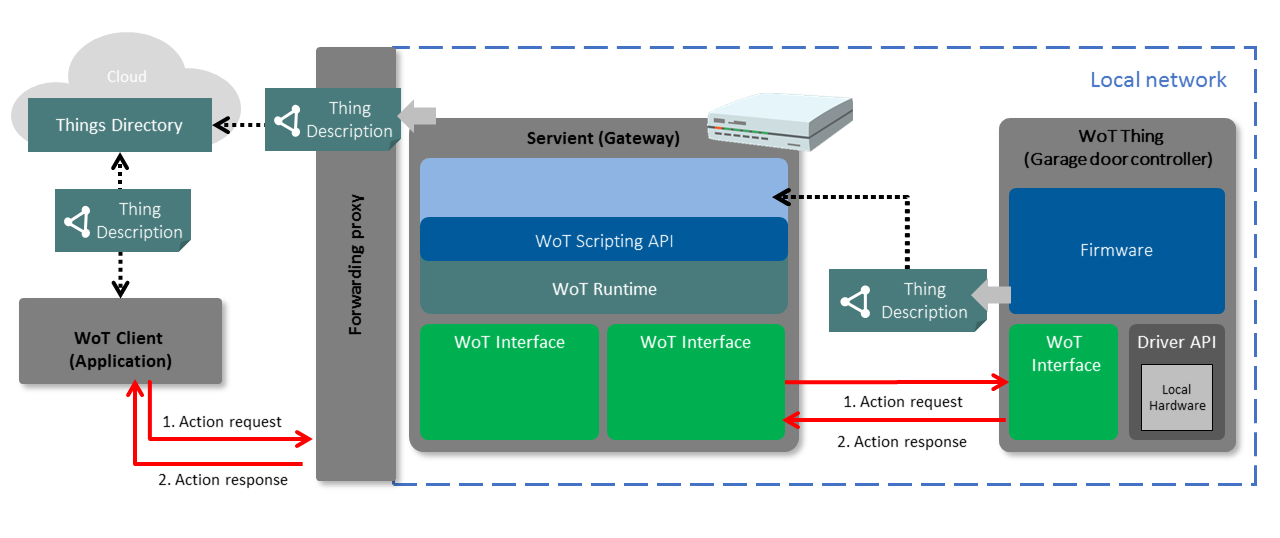
\includegraphics[width=6in]{figures/wot-scenario.png}
\caption{Typical WoT deployment scenario}
\label{fig-wot-scenario}
\end{figure*}

